\section{发电机}\label{sec:10-13}

法拉第发现的电磁感应现象的重要应用之一就是用来制成发电机。
发电机是把机械能转化成电能的机器,是当代社会中最重要的电源。

\begin{figure}[htbp]
    \centering
    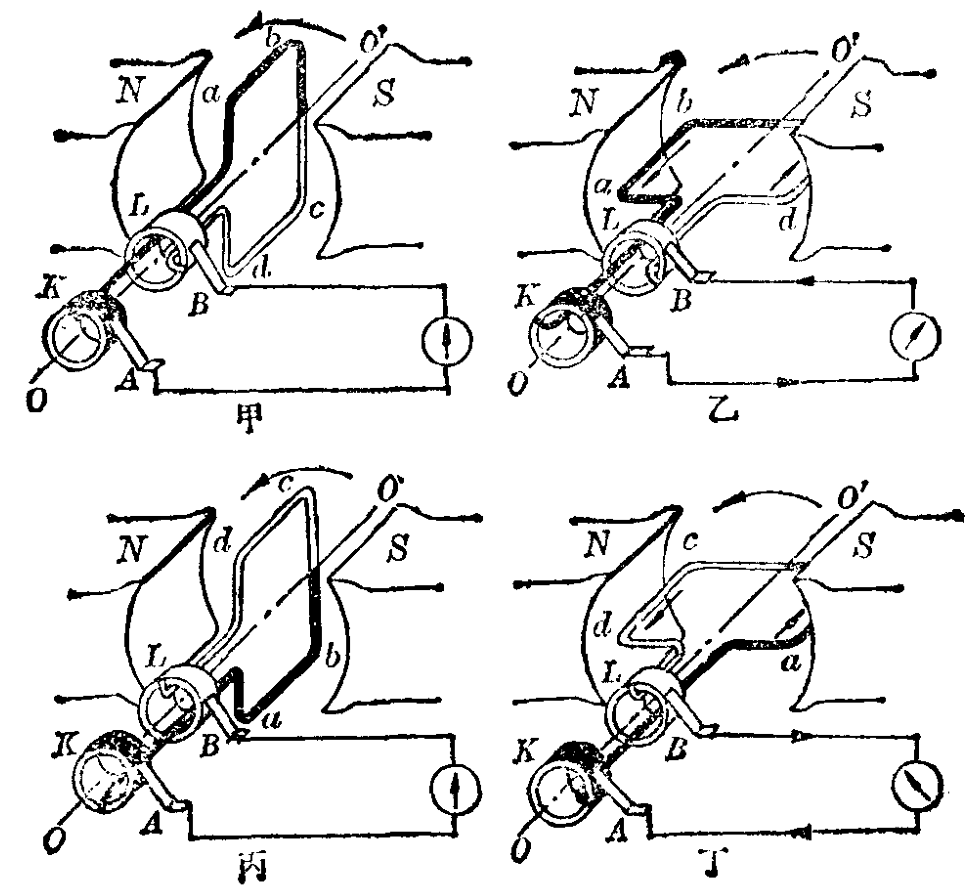
\includegraphics[width=0.7\textwidth]{../pic/czwl2-ch10-47}
    \caption{}\label{fig:10-47}
\end{figure}

图 \ref{fig:10-47} 是交流发电机的模型。矩形线圈 $abcd$ 可以绕轴 $oo'$ 转动,
$ab$ 边和 $cd$ 边分别接到铜滑环 $K$、$L$ 上,两个滑环又分别跟电刷 $A$ 和 $B$ 接触着。
用导线将电刷 $A$、$B$ 分别连接到电流表的两个接线柱上,组成闭合电路。
线圈转动时,由于 $ab$ 边和 $cd$ 边做切割磁力线运动,线圈中就产生感生电流。

当线圈逆着时针方向从图甲经图乙向图丙转的半周内,
$ab$ 边向下运动,$cd$ 边向上运动,根据右手定则,
$ab$ 边中的感生电流方向由 $b \to a$,
$cd$ 边中的感生电流方向由 $d \to c$。
外部电路中的电流方向是由电刷 $A$ 流向电刷 $B$,如图乙所示。
当线圈转过半周继续从图丙经图丁向图甲转的半周内,
$ab$ 边变为向上运动,$cd$ 边变为向下运动,
$ab$ 边中感生电流的方向变为由 $a \to b$,
$cd$ 边中感生电流的方向变为由 $c \to d$。
外部电路中的电流方向是由电刷 $B$ 流向电刷 $A$,如图丁所示。
线圈再从图甲的位置继续转动下去,感生电流将完全重复着上述变化。
因而线圈中感生电流的方向和外部电路中电流的方向都是周期性变化的。
这从电流计指针的左右摆动可以看出来。这种周期性地改变方向的电流叫做交流电。
这跟我们从干电池和蓄电池所得到的方向不变的直流电有所不同。

图 \ref{fig:10-47} 只是用来说明交流发电机的原理的,实际的交流发电机,结构很复杂。
但主要由定子(不动部分)和转子(运转部分)两部分组成。
为了使发电机发出很高的电压和很强的电流,大型发电机的线圈的匝数很多,导线也很粗。
要使巨大的线圈高速旋转,需要解决的技术问题比较复杂,
因此大型发电机采用线圈不动而磁场旋转的方式,把线圈嵌在定子铁心的槽里。
为了得到较强的磁场,用电磁铁代替永久磁铁作转子,由专用的直流电源经电刷、滑环给电磁铁供电。

实际用的发电机,它的转子是由水轮机、汽轮机、内燃机等发动机带动的,
发电机把这些发动机供给的机械能转化为电能。
彩图8 为水电站厂房内景,图中看到的是一排大型发电机,带动这些发电机的水轮机,都在厂房地面下面。

\begin{figure}[htbp]
    \centering
    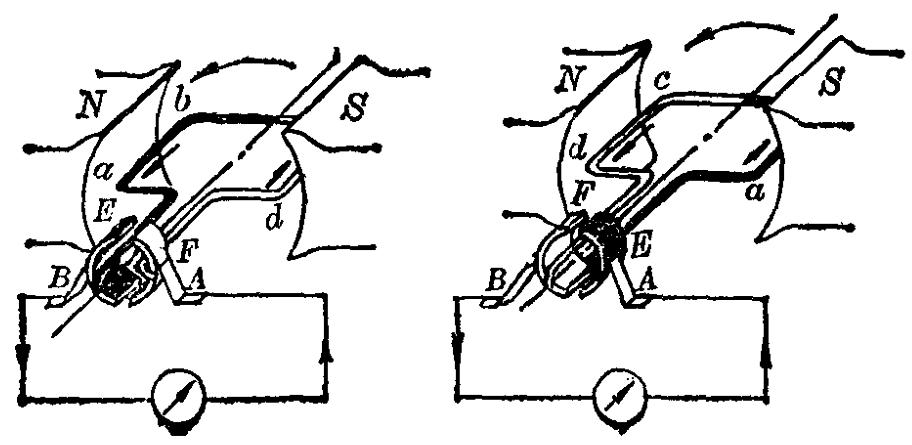
\includegraphics[width=0.8\textwidth]{../pic/czwl2-ch10-48}
    \caption{}\label{fig:10-48}
\end{figure}

除了交流发电机,还有直流发电机。图 \ref{fig:10-48} 表示直流发电机的原理。
它用换向器来代替交流发电机上的两个铜滑环。
这样,虽然线圈中产生的是交流电,而供给外部电路的却是直流电。

